\subsection{Development Process} \label{Development Process section}
\almarginpar{How is the development process related to the research design and its process defined in Fig 9}
The minimum viable artefact is a Python notebook file containing Python scripts to run the experiment.
We run the notebook with IBM Quantum Experience, as they provide online services for simulating quantum hardware.
\almarginpar{You need to show that you have followed your research design}
The following sections describe our experimental process.

\subsubsection{The Quantum Emulator}
For this experiment, we are using the quantum emulator provided by Qiskit.
The QASM simulator is used to mimic an IBMQ device.
\almarginpar{Fault free runs are not exactly simulating the quantum device, any comment or justification? Perhaps future work?}
Additionally, QASM simulator by default has no noise, so we can expect the result to be noise-free.

\subsubsection{Creating Ansatzes}
\almarginpar{Which of the ansatze would be most useful to support QNN? Wouldn't RealAmplitudes be useful for "real" QNN implementation?}
We have chosen two ansatzes \textit{NLocal} and \textit{TwoLocal} from the Qiskit circuit library due to their wide usage in quantum machine learning.
As discussed in the Research Design section \ref{Research Design section}, we configure the ansatz objects such that initially their gradient variances decrease exponentially with the number of qubits.
These characteristics are:
\begin{itemize}
    \item The circuit depth;
    \item The number of qubits to be measured for the cost function;
    \item The randomised parameters.
\end{itemize}

An example of circuits generated by Qiskit is visualised in Figure \ref{Ansatz samples}.
By altering the repetition number and qubit number, we can generate different ansatz.
The circuit depth is the largest number of gate operations across all qubit registers in a circuit. 
Furthermore, as the circuit high-level definition is translated into the gate set available on a given quantum machine, the circuit depth may significantly increase.
Obviously, as the ansatz repetition grows, the circuit depth also grows.
Figure \ref{Ansatz samples} further shows that for a fully entangled ansatz, the higher number of qubits also leads to deeper circuit.

\begin{figure}
    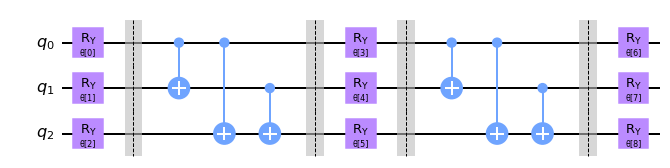
\includegraphics[width=\textwidth]{Artefact/Appendices/ansatz3-2.png}
    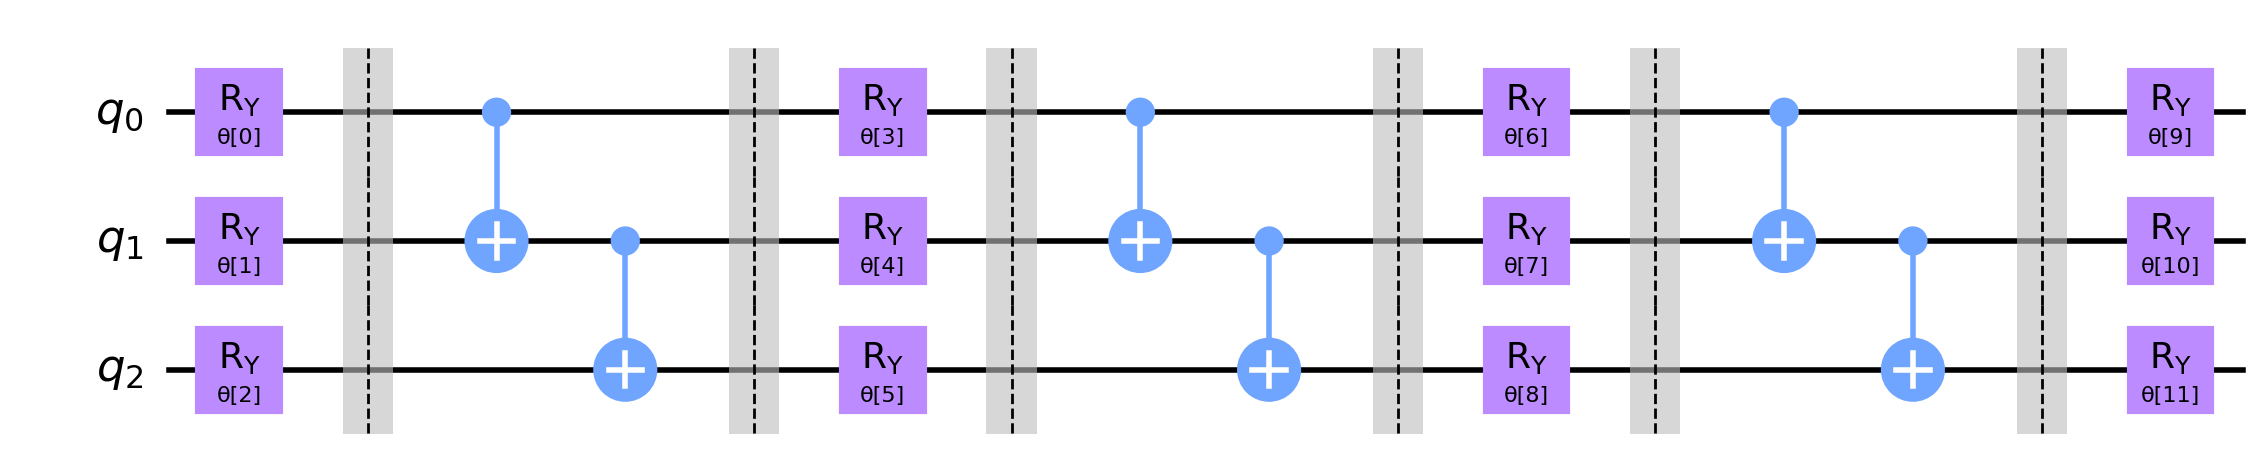
\includegraphics[width=\textwidth]{Artefact/Appendices/ansatz3-3.png}
    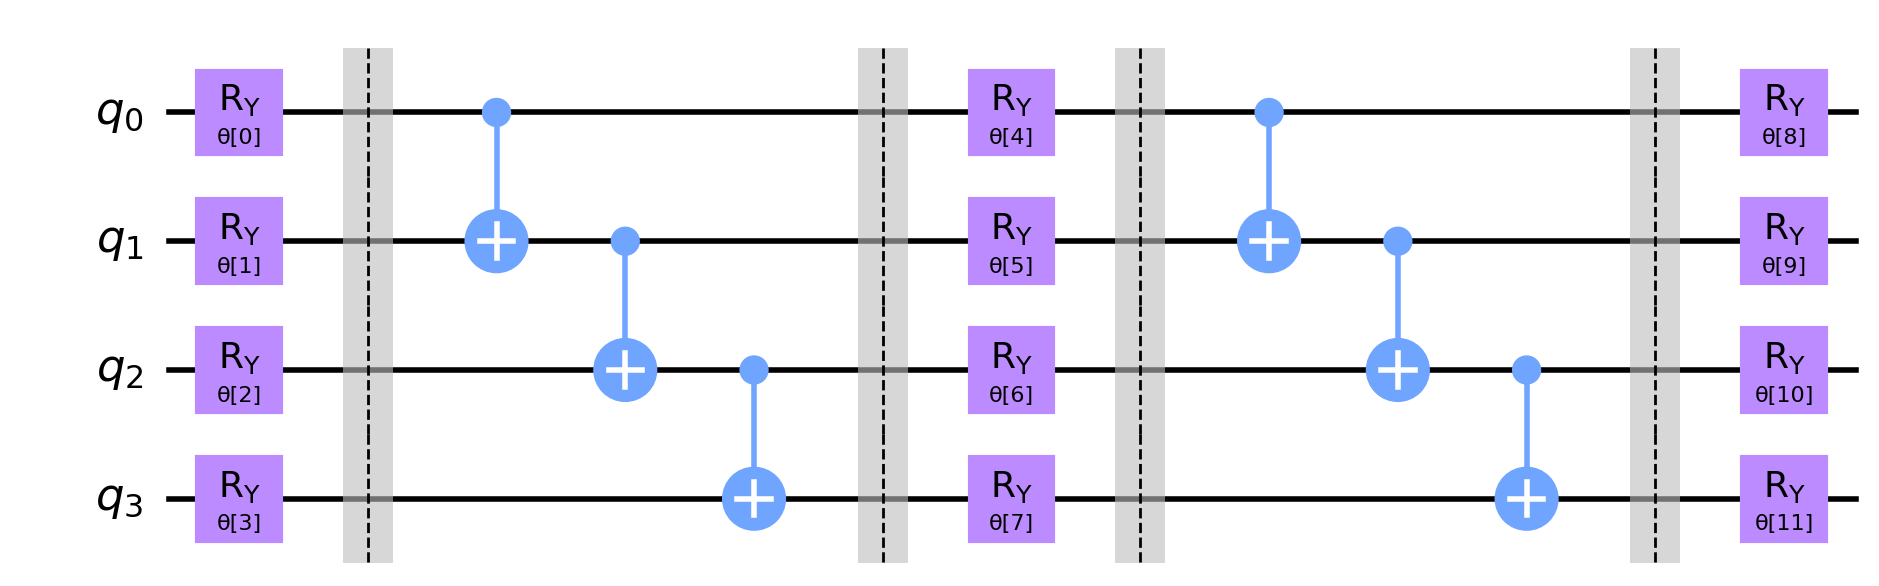
\includegraphics[width=\textwidth]{Artefact/Appendices/ansatz4-2.png}
    \caption{
        Samples of parameterised circuits generated by the Qiskit framework with 'full entanglement' option.
        The ansatz is a sequence of rotation layers and entanglement layers.
        Above: an ansatz of three qubits and two repetition layers.
        Middle: an ansatz of three qubits and three repetition layers.
        Below: an ansatz of four qubits and two repetition layers.
    }
    \label{Ansatz samples}
\end{figure}

\subsubsection{Visualise the Variance}
To calculate the gradient variance, we use the parameter shift rule from Eq. (\ref{Parameter-shift rules}) as implemented in Qiskit Gradient Framework.
The BP phenomena can be verified when the gradient variance decreases with an increased number of qubits and repetition layers.

To visualise the gradient variances, we have plotted a range of random parameters for each ansatz as the initial starting point.
Such randomised parameters are generated 100 times uniformly to calculate the gradients.
We then plot the variance values of the gradients for different numbers of qubits and repetition values for a range of 2 to 9 qubits and ansatz layer repetition.
Note that the neural network generated in this experiment is not designed to answer a problem, we will focus on the trainability of each method in later steps of the experiment.

In short, we use 100 uniformly randomised parameters to scan the gradient, then we calculate the "slope" of the gradient.

\subsubsection{Experiment with Local Cost Function and Shallow Depth}
The two ansatzes are configured such that their depths are fixed, along with a local cost function.
The \textit{Global Cost Function} is the combined output of all qubits. 
On the other hand, the \textit{Local Cost Function} only compares the values of individual qubits or a subset of qubits \cite{cerezoCostFunctionDependent2021}.
Section \ref{Shallow Circuits, Local Cost Function section} and figure \ref{cost functions} previously explained the differences between the two cost functions.

\almarginpar{There is some repetition between the first and the second paragraph, improve!}
We implemented the global cost function as the measurement output for all qubits, while the local cost function is the measurement for the first two qubits.
\almarginpar{I do not get the logic and the motivation - the number of repetions = number of qubits? Why? The whole paragraph may need to be clarified - I do not understand!}
We define the deep circuit as the circuit that scales with the number of qubits and the number of repetition, we implement the default ansatz to have the number of qubits equal to the number of repetition in a fully entangled configuration. 
The shallow ansatz is the same as compared with the default, however, the repetition number is kept as a constant number.